\documentclass[thesis.tex]{subfiles}
\renewcommand\_{\textunderscore\allowbreak}

\begin{document}
\chapter{Datasets and Triggers}
\label{ch4}

\section{Datasets}
\label{sec:dataandsimulation}
This search is based on a data sample corresponding to an integrated luminosity of 35.9 $fb^{-1}$ of proton-proton collisions at $\sqrt{s} =$ 13 TeV produced by the LHC in 2016.
The analysis is performed in both the $e + \gamma$ and $\mu + \gamma$ channels. 
Events in each channel  are selected from the corresponding primary dataset with dedicated lepton plus photon triggers.
Monte-Carlo (MC) simulated events are also used for various purpose.  

\subsection{Data}
Reconstructed data sets of the CMS are further skimmed by event filters to keep only the information needed by physics analysis. 
These samples with reduced file size are called miniAOD~\cite{miniAOD}. 
Events of this analysis are selected from the miniAOD datasets produced with the CMS software framework, CMSSW\_8\_0\_26\_patch1.
A total of 35.9 $fb^{-1}$ of data was certified to be good for physics analysis. The ``golden JSON'' file 
Cert\_271036-284044\_13TeV\_23Sep2016ReReco\_Collisions16\_JSON.txt, which provides a list of run numbers and lumi section numbers of data with good quality, is used to select the certified datasets. 

The candidate $e\gamma$ events are selected out of the DoubleEG primary dataset with the diphoton trigger: HLT\_Diphoton30\_18\_R9Id\_OR\_IsoCaloId\_AND\_HE\_R9Id\_Mass90. 
The $\mu\gamma$ events are selected from the MuonEG dataset, triggered by either the HLT\_Mu17\_Photon30\_CaloIdL\_L1Iso or HLT\_Mu38NoFilterNoVtx\_Photon38\_CaloIdL. 
In addition, SingleMuon and SingleElectron datasets are used in this analysis for various backgrounds estimation and efficiency measurements. 
The datasets used in this analysis are summarized in Table~\ref{tab:datasettab}. \\

\begin{table}[htbp]
\begin{center}
  \caption{Datasets used in this analysis.}
   \label{tab:datasettab}
  \begin{tabular}{ | c| c | }
     \hline 
    Primary Dataset & Samples \\ \hline
     \multirow{8}{*}{DoubleEG} & /DoubleEG/Run2016B-03Feb2017\_ver2-v2/MINIAOD \\ 
                      & /DoubleEG/Run2016C-03Feb2017-v1/MINIAOD  \\
                      & /DoubleEG/Run2016D-03Feb2017-v1/MINIAOD   \\ 
                      & /DoubleEG/Run2016E-03Feb2017-v1/MINIAOD   \\ 
                      & /DoubleEG/Run2016F-03Feb2017-v1/MINIAOD   \\ 
		     & /DoubleEG/Run2016G-03Feb2017-v1/MINIAOD   \\
		     &  /DoubleEG/Run2016H-03Feb2017\_ver*-v1/MINIAOD \\ \hline
      \multirow{8}{*}{MuonEG}  & /MuonEG/Run2016B-03Feb2017\_ver2-v2/MINIAOD \\
                      & /MuonEG/Run2016C-03Feb2017-v1/MINIAOD  \\
                      & /MuonEG/Run2016D-03Feb2017-v1/MINIAOD   \\ 
                      & /MuonEG/Run2016E-03Feb2017-v1/MINIAOD   \\ 
                      & /MuonEG/Run2016F-03Feb2017-v1/MINIAOD   \\ 
		     & /MuonEG/Run2016G-03Feb2017-v1/MINIAOD   \\
		     & /MuonEG/Run2016H-03Feb2017\_ver*-v1/MINIAOD \\ \hline
    \multirow{8}{*}{SingleElectron}   & /SingleElectron/Run2016B-03Feb2017\_ver2-v2/MINIAOD \\ 
                     & /SingleElectron/Run2016C-03Feb2017-v1/MINIAOD  \\
                     & /SingleElectron/Run2016D-03Feb2017-v1/MINIAOD   \\ 
                     & /SingleElectron/Run2016E-03Feb2017-v1/MINIAOD   \\ 
                     & /SingleElectron/Run2016F-03Feb2017-v1/MINIAOD   \\ 
		     & /SingleElectron/Run2016G-03Feb2017-v1/MINIAOD   \\
		     & /SingleElectron/Run2016H-03Feb2017\_ver*-v1/MINIAOD \\ \hline
     \multirow{8}{*}{SingleMuon} & /SingleMuon/Run2016B-03Feb2017\_ver2-v2/MINIAOD \\
                & /SingleMuon/Run2016C-03Feb2017-v1/MINIAOD  \\
                & /SingleMuon/Run2016D-03Feb2017-v1/MINIAOD   \\ 
                & /SingleMuon/Run2016E-03Feb2017-v1/MINIAOD   \\ 
                & /SingleMuon/Run2016F-03Feb2017-v1/MINIAOD   \\ 
		& /SingleMuon/Run2016G-03Feb2017-v1/MINIAOD   \\
		& /SingleMuon/Run2016H-03Feb2017\_ver*-v1/MINIAOD \\ \hline
     \end{tabular}
     \end{center}
 \end{table}   

\subsection{Simulation}
MC simulated events are used in this analysis to study the search strategy, model the SUSY signal yields, estimate the background contributions, and validate the analysis methods.
All the MC simulation samples are listed in Table \ref{Tab:2}, along with the cross-sections calculated at the same perturbative order as the generator. 

\begin{table}[ht]	
\begin{center}
  \caption{List of the MC samples used for signal and SM background processes, with their cross-sections and corresponding equivalent integrated luminosity. [13TeV] stands for TuneCUETP8M1\_13TeV-amcatnloFXFX-pythia8, and [S16] stands for RunIISummer16MiniAODv2-PUMoriond17\_80X\_mcRun2\_asymptotic\_2016\_TrancheIV\_v6. }\label{Tab:2}
  \resizebox{\linewidth}{!}{
  \begin{tabular}{ | c| c | c | c | }
     \hline 
    Process & Samples & $\sigma$(pb) & \texorpdfstring{$\mathcal{L}_{eff}$}(fb$^{-1}$)  \\ \hline \hline
                & /SMS-T5Wg\_[13TeV]/RunIISpring16MiniAODv2-PUSpring16Fast\_  & - & - \\
    SUSY   & 80X\_mcRun2\_asymptotic\_2016\_miniAODv2\_v0-v1/MINIAODSIM  & & \\  \cline{2-4}
                & /SMS-TChiWG\_[13TeV]/RunIISpring16MiniAODv2-PUSpring16Fast\_  & - & - \\
                	& 80X\_mcRun2\_asymptotic\_2016\_miniAODv2\_v0-v1/MINIAODSIM  & &  \\  \hline
    \hline
    $W\gamma$ & /WGToLNuG\_TuneCUETP8M1\_13TeV-madgraphMLM-pythia8/[S16]-v1/MINIAODSIM & 337 & 18.11  \\ \cline{2-4}
                          & /WGJets\_MonoPhoton\_PtG-40to130\_TuneCUETP8M1\_13TeV-madgraph/[S16]-*/MINIAODSIM & 12.5 & 409 \\  \hline
                          & /WGJets\_MonoPhoton\_PtG-130\_TuneCUETP8M1\_13TeV-madgraph/[S16]-*/MINIAODSIM & 0.64 &  3.6e+03 \\  \hline
    $Z\gamma$   & /ZGTo2LG\_[13TeV]/[S16]\_ext1-v1/MINIAODSIM   &  117.864 & 121.9   \\ \cline{2-4}
    $t\bar{t}\gamma$ & /TTGJets\_[13TeV]-madspin-pythia8/[S16]\_ext1-v1/MINIAODSIM & 3.697 & 1.32e+03  \\ \hline
    $t\bar{t}$  &  /TTJets\_[13TeV]-madgraphMLM-pythia8/[S16]-v1/MINIAODSIM & 502.2 & 20.19 \\ \hline
    $WW$        & /WW\_TuneCUETP8M1\_13TeV-pythia8/[S16]\_ext1-v1/MINIAODSIM & 63.21 & 110.53 \\ \hline
    $WZ$        & /WZ\_TuneCUETP8M1\_13TeV-pythia8/[S16]\_ext1-v1/MINIAODSIM & 22.82 & 131.28 \\ \hline
    $WW\gamma$  &  /WWG\_[13TeV]/[S16]\_ext1-v1/MINIAODSIM & 0.2147 &  4.65e+03 \\ \hline
    $WZ\gamma$  &  /WZG\_[13TeV]/[S16]-v1/MINIAODSIM & 0.04123 & 2.42e+04 \\ \hline
    $DY$       & /DYJetsToLL\_M-50\_[13TeV]/[S16]\_ext2-v1/MINIAODSIM  & 5670 & 21.5 \\ \hline
  \end{tabular}
  }
  \end{center}
\end{table}   

The SM processes are generated with MadGraph\_aMC@NLO 2.3.3~\cite{madgraph233} in the CMS Moriond17 campaign, except for the W+$\gamma$ samples which are generated with MadGraph in leading order (LO). 
To correct the W+$\gamma$ cross-section, a constant NNLO k-factor of 1.34 is applied \cite{K:MonoPho, K:Bozzi}.
All samples use the NNPDF 3.0~\cite{pdfNNPDF} parton distribution functions (PDFs). 
The hard scattering processes  are interfaced to Pythia 8.2~\cite{pythia82} with the CUETP8M1 generator tune~\cite{cmstune} for simulation of parton showers,  hadronization and decays. 
Detector simulations are performed with a Geant4~\cite{Agostinelli:2002hh} based package which has a detailed description of the CMS detector. 
Simulated events are digitized and reconstructed by the same algorithms that are used for real collision data. 

The pile-up contribution is also considered in MC samples by superimposing minimum bias events on the simulated events. 
To mitigate the possible mismodeling of pile-up profile in simulations, the MC events are reweighted such that the number of vertices has the same distribution as measured in data, as shown in Figure \ref{fig:PUreweight}.

\begin{figure}[tb]
  \centering
    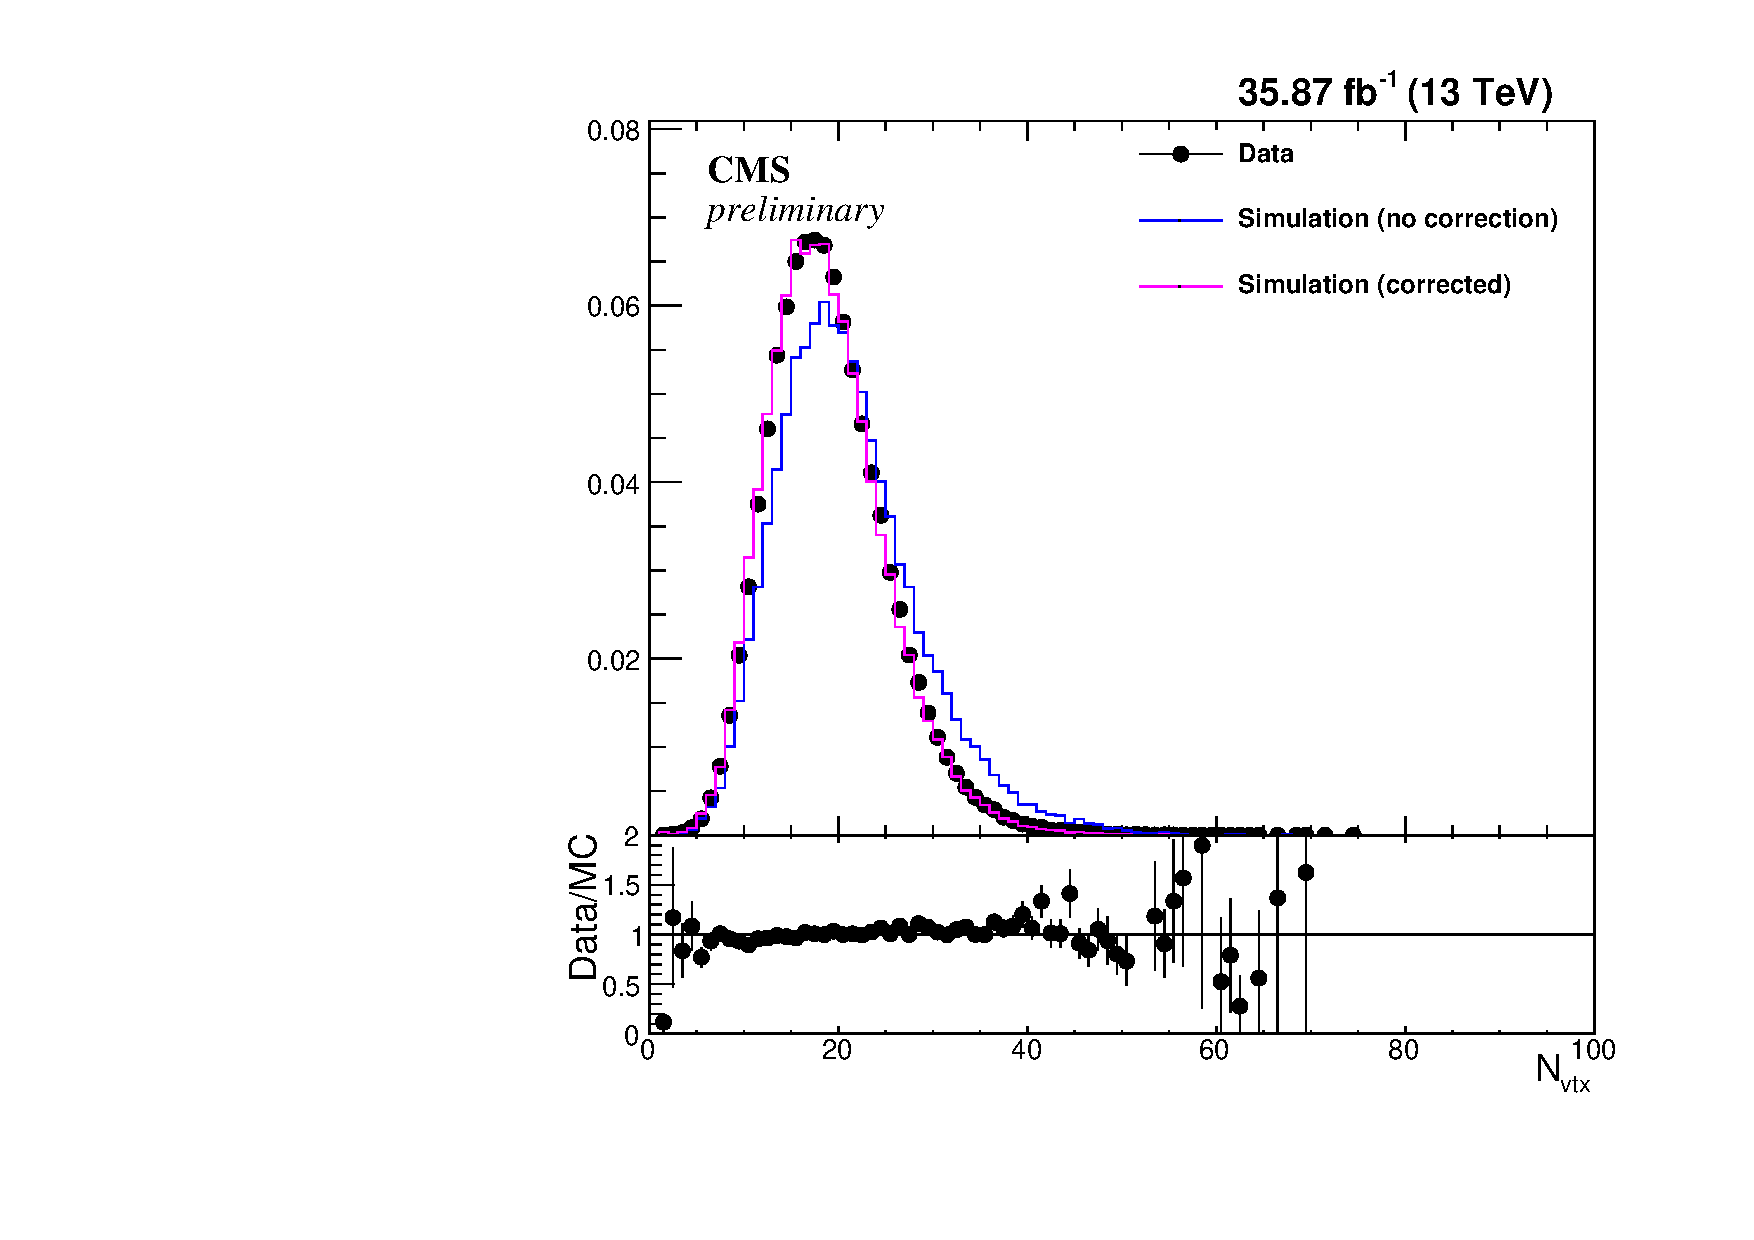
\includegraphics[width=0.8\textwidth]{Figures/PLOT_PUreweight.pdf}
  \caption{The distribution of the number of reconstructed vertices for data (black dots) and simulation (solid lines). The simulated events before (blue) and after (magenta) the pile-up reweighting are shown. The lower panel shows the ratio between the reweighted simulation and data.} 
  \label{fig:PUreweight}
\end{figure}


\section{Trigger}
\label{sec:trigger}
A diphoton trigger, HLT\_Diphoton30\_18\_R9Id\_OR\_IsoCaloId\_AND\_HE\_R9Id\_Mass90\_v*, is used to collect the signal candidate events for the $e\gamma$ channel. Each HLT diphoton path is seeded from the logic OR of a list of L1 EG triggers.
For the $\mu\gamma$ channel, a muon-photon trigger, HLT\_Mu17\_Photon30\_CaloIdL\_L1Iso\_v*, is used for events selection. 
HLT\_Mu38NoFilterNoVtx\_Photon38\_CaloIdL is used in addition with logic OR to compensate for possible trigger inefficiencies caused by the isolation requirement in L1 EG seed. 
A summary of the signal HLT paths with their L1 seeds is shown in Table \ref{Tab:3}. 
The measurement of trigger efficiencies is described in subsequent sections.

\begin{table}[ht]	
\begin{center}
  \caption{List of the HLT used for signal selections.}\label{Tab:3}
 \resizebox{\linewidth}{!}{
  \begin{tabular}{ | c| c | c |  }
     \hline 
     Channel & HLT & L1 seed \\ \hline
     $e\gamma$ & HLT\_Diphoton30\_18\_R9Id\_OR\_IsoCaloId\_AND\_HE\_R9Id\_Mass90\_v* &  L1\_SingleEG* \\
     	 & &  OR L1\_SingleIsoEG* \\
     	 & &  OR L1\_DoubleEG\_* \\ \hline
     $\mu\gamma$ & HLT\_Mu17\_Photon30\_CaloIdL\_L1Iso\_v* & L1\_Mu5IsoEG18  \\
     					&  & OR L1\_Mu5IsoEG20  \\ \cline{2-3}
     			    & HLT\_Mu38NoFilterNoVtx\_Photon38\_CaloIdL & L1\_Mu5EG20\\
     			    &   & OR L1\_Mu20EG15 \\ \hline
     \end{tabular}
   }
  \end{center}
\end{table}   

\subsection{$e\gamma$ Trigger Performance}
The diphoton HLT path doesn't veto events if one or more photons have associated tracks. 
Therefore this path allows the $e+\gamma$ events to be triggered.
The diphoton HLT is seeded from a combination of various L1 EG triggers to achieve an optimal L1 efficiency. 
The leading leg of the HLT is then reconstructed around the L1 seed and required to pass the following quality filters: 
\begin{itemize}
	\item $E_T > $ 30 GeV, $|\eta| < $ 2.5
	\item $R_{9 (5\times5)} >$ 0.5(0.8) in EB(EE), where $R_{9(5\times5)}$ is the energy sum of $3\times3$ crystals centered on the cluster seed divided by that of $5\times5$ crystals.
	\item H/E $<$ 0.12 (0.1) in EB(EE)
	\item Either $\sigma_{i\eta i\eta} <$ 0.015 (0.035) in EB(EE), ECAL isolation $<$ 6.0 + 0.012$E_T$ \\
		OR $R_{9 (5\times5)} >$ 0.85 (0.9)
\end{itemize}

If the leading leg passes these kinematic and shower quality filters, the entire ECAL data will be reconstructed. 
In the unseeded step, at least two clusters are required to have $E_T > $ 18 GeV and pass the unseeded filters, which have the same criteria with the seeded leg and in addition a cut on the track isolation. 
The final trigger requires the diphoton mass to be greater than 90 GeV. The total efficiency is given by:
\begin{eqnarray*}
	\epsilon_{diphoton} = \epsilon_{sub, sub} \cdot \epsilon_{lead, sub} \cdot \epsilon_{lead, lead},
\end{eqnarray*}
where $\epsilon_{lead, lead}$ is the efficiency of matching the leading photon to the seeded leg object, $\epsilon_{lead, sub}$ is the efficiency for the leading photon to pass the unseeded filters, and $ \epsilon_{sub, sub}$ is the efficiency of matching the sub-leading photon to an unseeded object. 

Because photons and electrons have similar ECAL cluster shapes, the diphoton trigger efficiency can be measured with a tag-and-probe method using the electron pairs from Z decays. 
Events are selected from the SingleElectron dataset using HLT\_Ele27\_eta2p1\_WPLoose\_Gsf, where the tag electron is required to match the single electron trigger leg and the probe object remains unbiased. 
The tag is a tightly selected electron with $p_T >$ 30 GeV.  
The probe is a photon passing the full offline selections except that the probe is allowed to have an associated pixel seed.
The tag and probe pair must have an invariant mass between 80 GeV and 100 GeV. 
The total number of selected probe objects is used as the denominator for the efficiency calculation, whereas the number of probes which can match leading leg objects of the diphoton HLT within $\Delta R <$ 0.3 is used as the numerator. 

The tag and probe pairs are used a second time for the sub-leading leg efficiency measurement. 
Since the sub-leading leg only gets reconstructed when a leading leg exists, the tag is required to match both the single electron trigger leg and the diphoton leading leg. 
The probe in this measurement is defined as a medium working point electron that passes all the offline selections described in section \ref{sec:eventSelection}. 
Out of such denominator electrons, those that have the sub-leading leg matched are counted as numerators. 
The trigger efficiency of probe photons and electrons are shown in Figure \ref{fig:egtriggereff}.

\begin{figure}[tb]
  \centering
    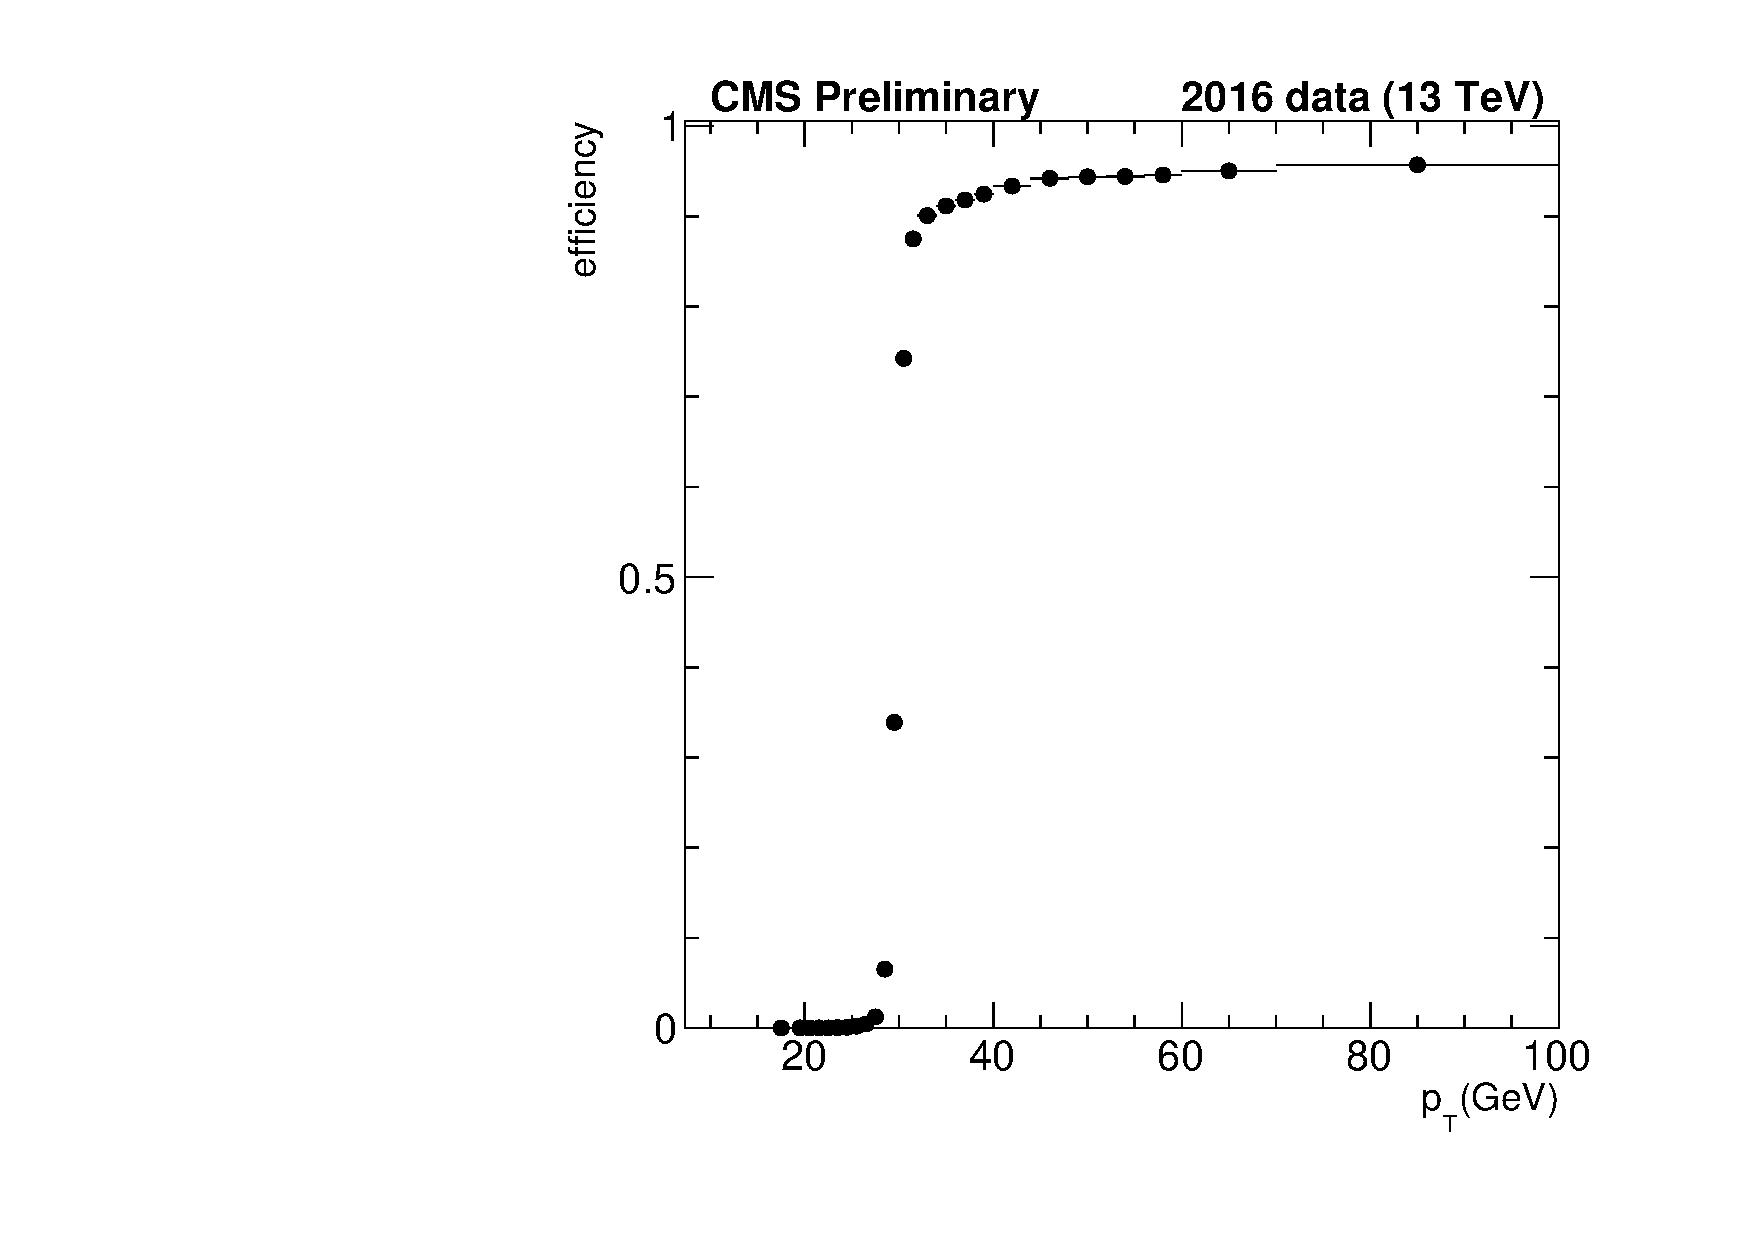
\includegraphics[width=0.49\textwidth]{Figures/egTrigger_2016_leading.pdf}\\
    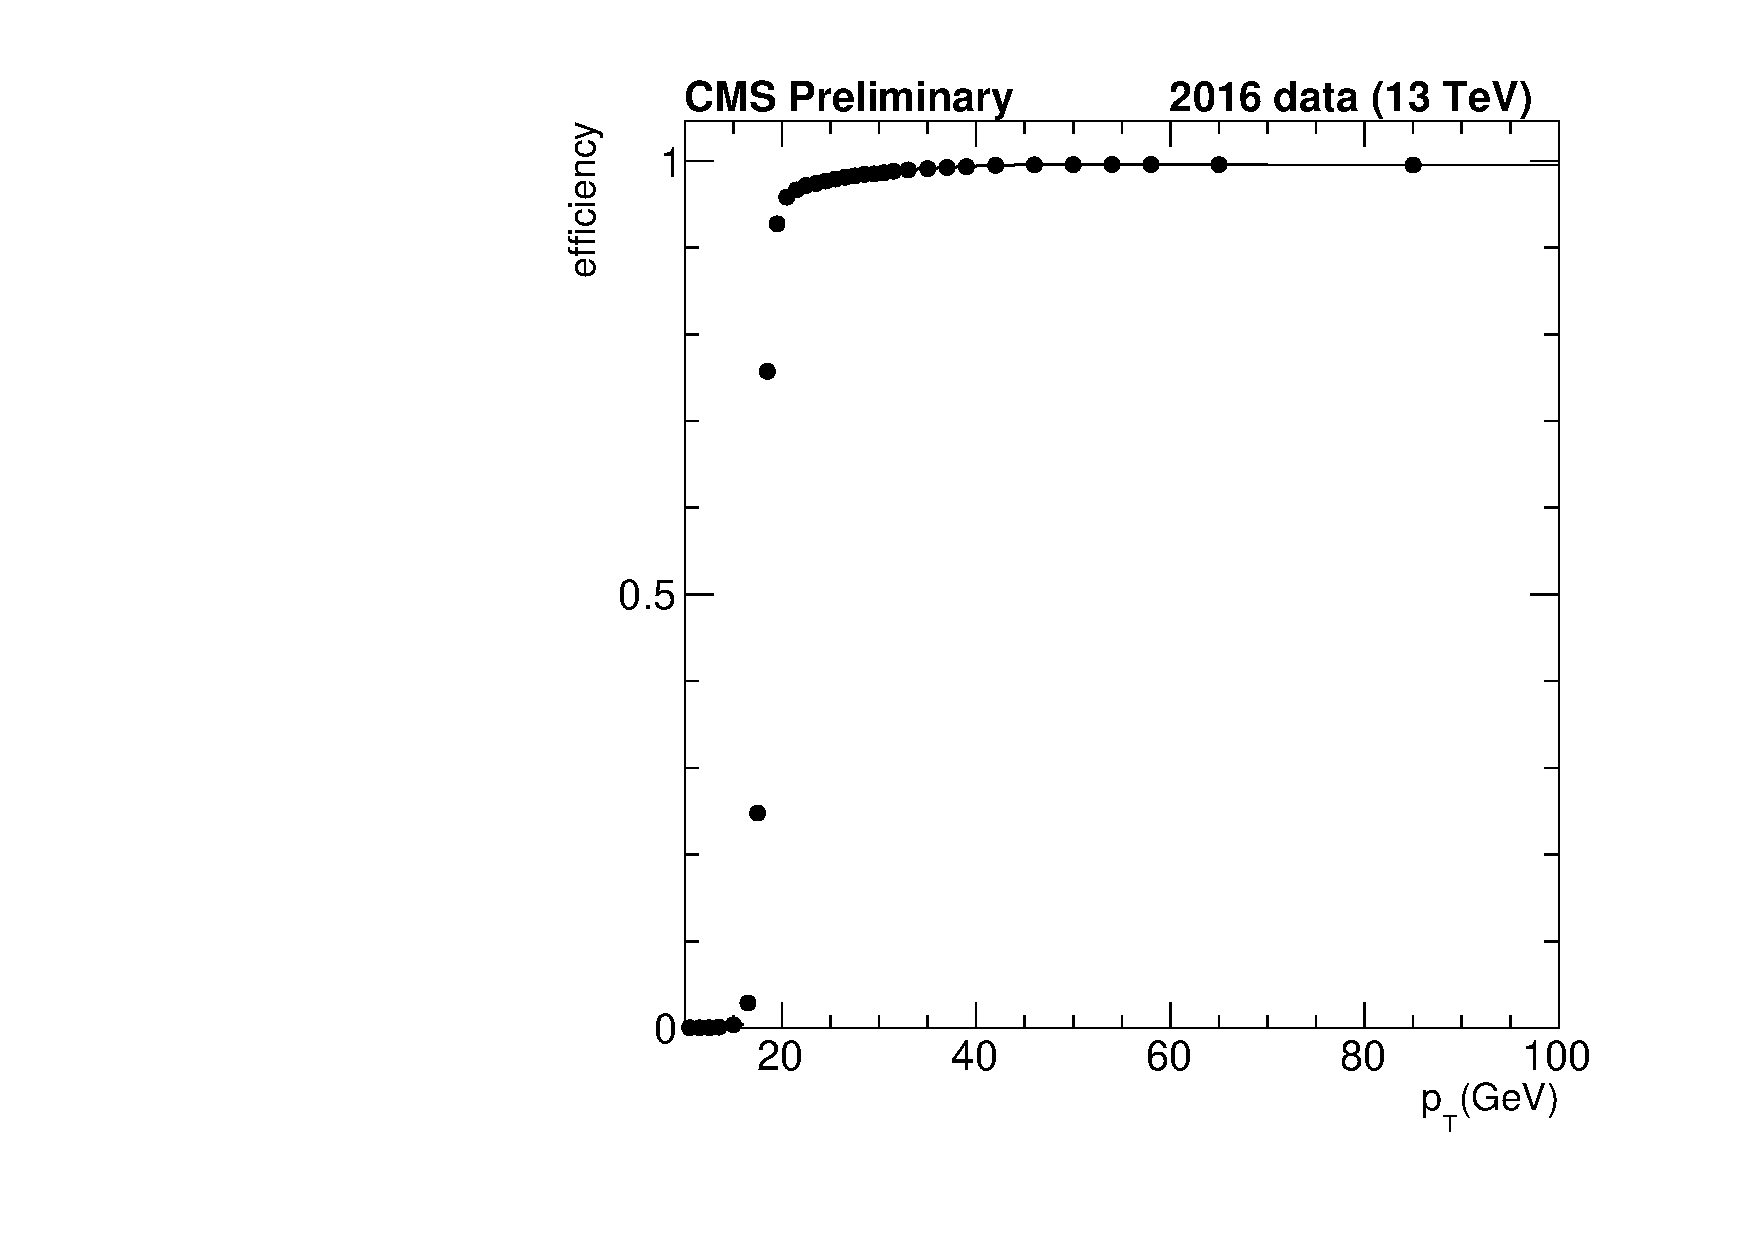
\includegraphics[width=0.49\textwidth]{Figures/egTrigger_2016_trailingEB.pdf}
    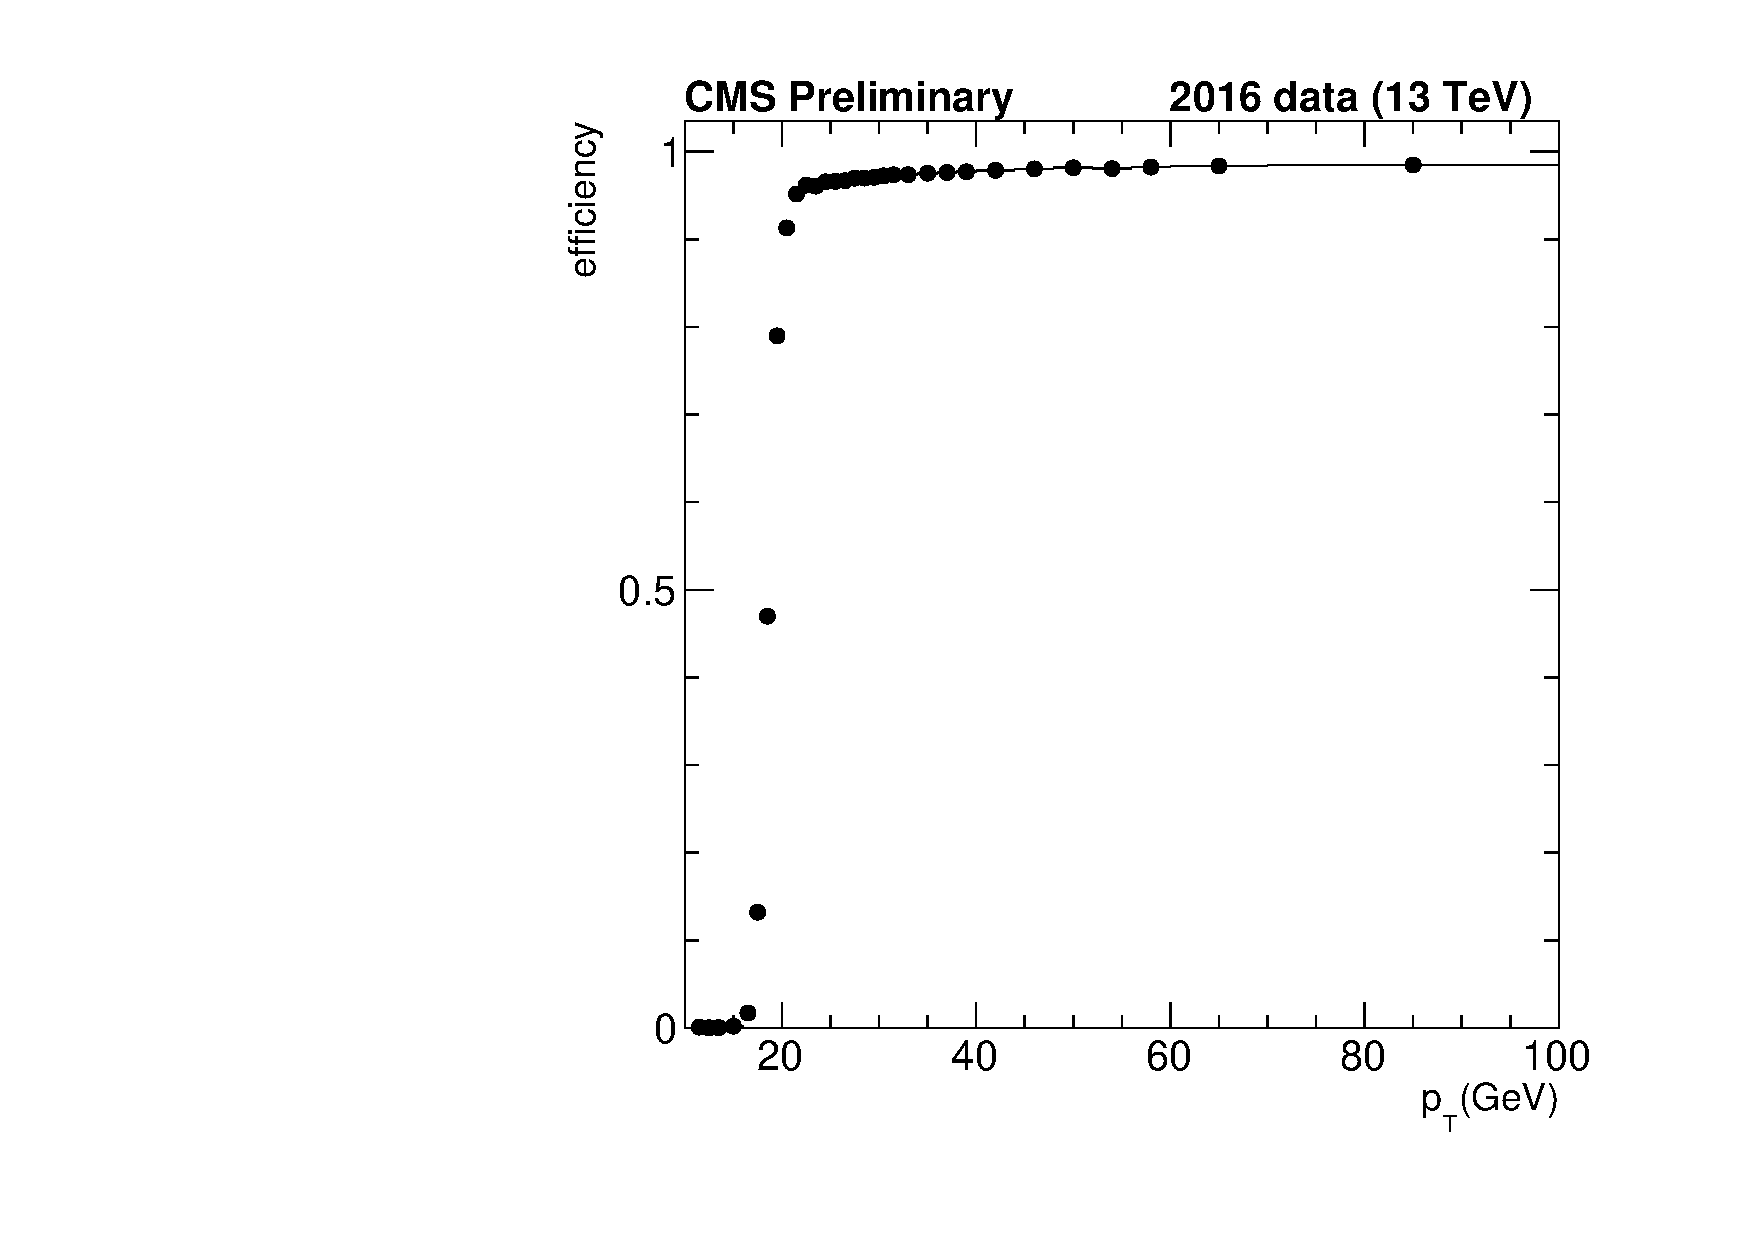
\includegraphics[width=0.49\textwidth]{Figures/egTrigger_2016_trailingEE.pdf}
  \caption{Trigger efficiencies for $e\gamma$ channel. Top: leading leg efficiency, bottom left: sub-leading leg efficiency (EB), bottom right: sub-leading leg efficiency (EE).}
  \label{fig:egtriggereff}
\end{figure}

In simulation, the identity of an object can be checked by geometrically matching it to a generated particle. 
This method is called MC truth-matching. 
Thus the trigger efficiency of simulated sample is derived by selecting the photon and electron with truth-matching and counting the number of objects which match the trigger legs. 
The efficiency measured in MC is then compared with that in data, and their ratio, $R = \epsilon^{data}/\epsilon^{MC}$ is used as the data-to-simulation trigger efficiency scale factor (ESF). 
Figure \ref{fig:egtriggerESF} shows the ESF of the photon and electron as a function of $p_{T}$ and $\eta$. 
Systematic uncertainties of the ESF are calculated from the tag-and-probe fits to the Z-peak. 

\begin{figure}[tb]
  \centering
  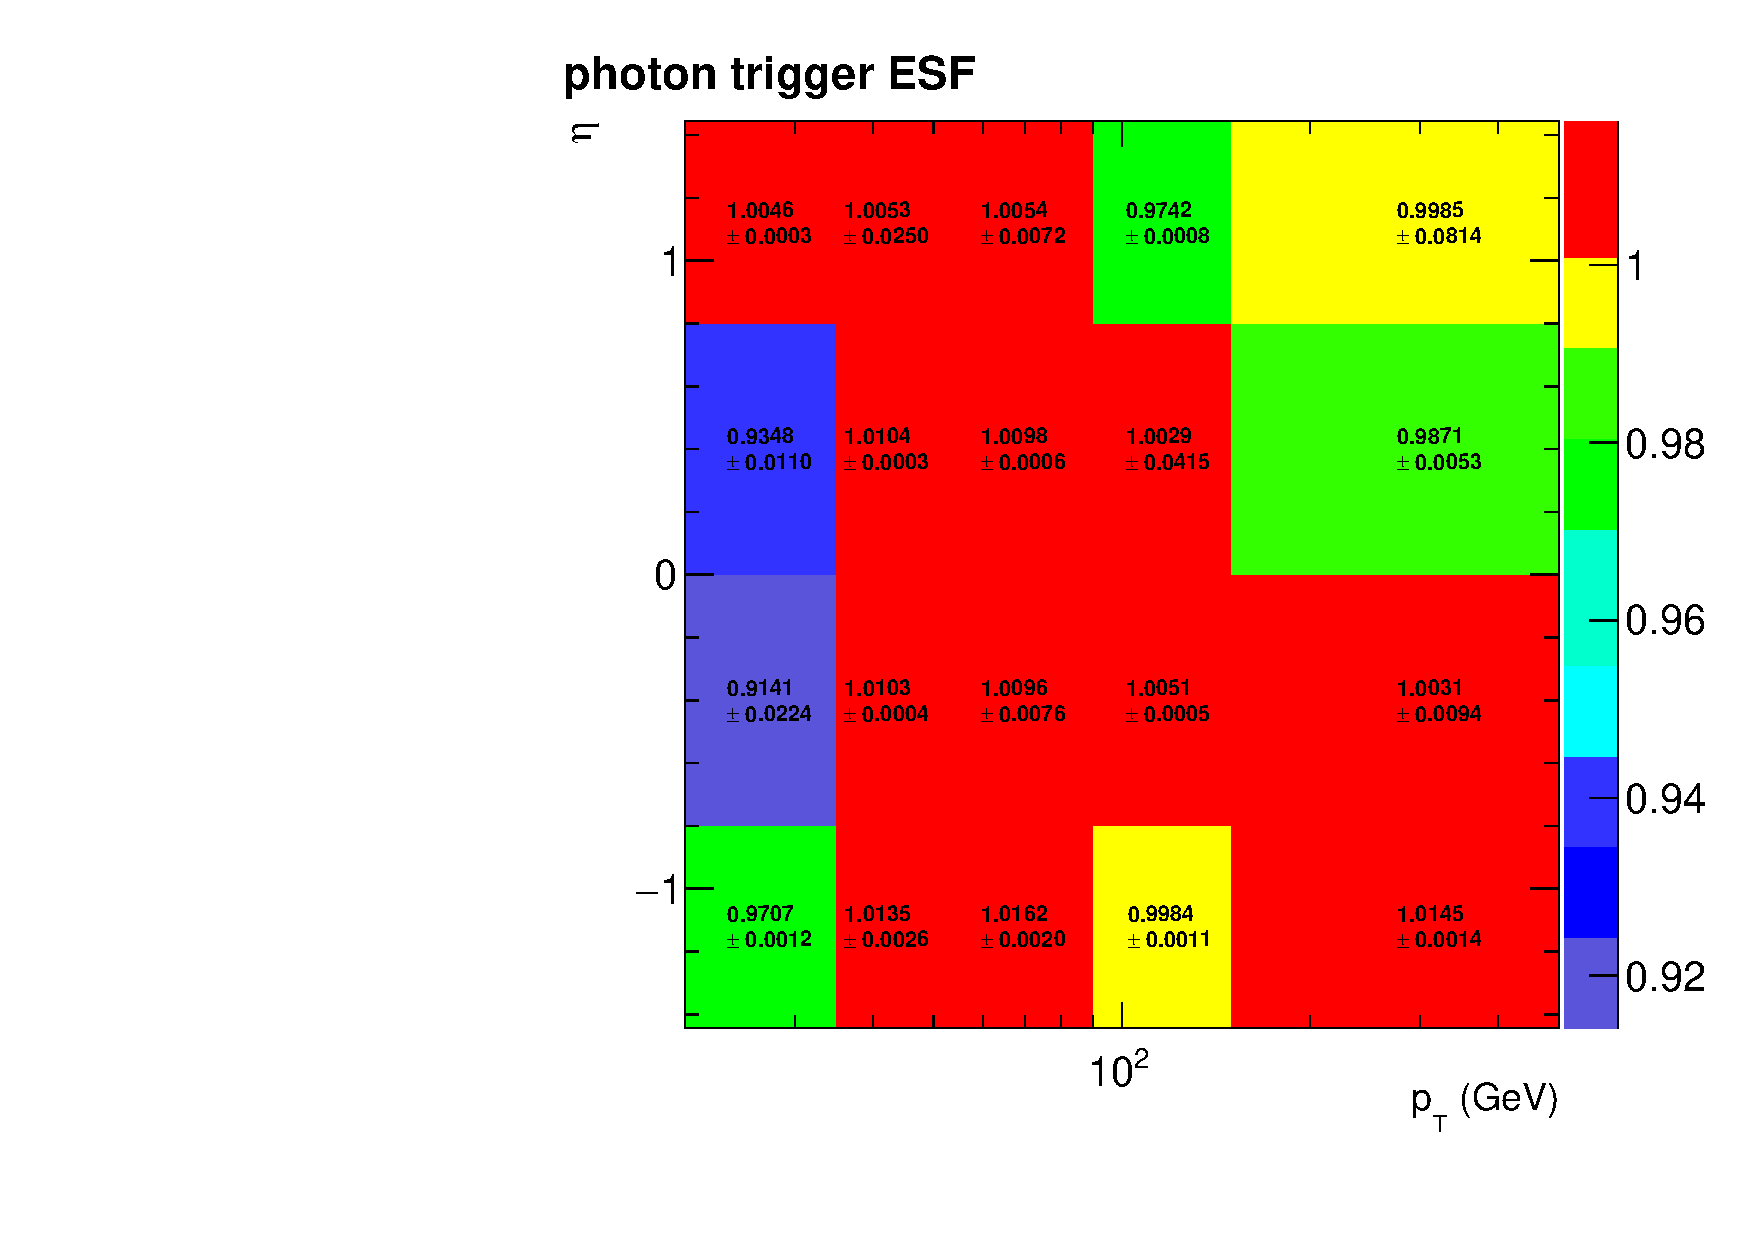
\includegraphics[width=0.49\textwidth]{Figures/egTrigger_LeadingESF.pdf}
  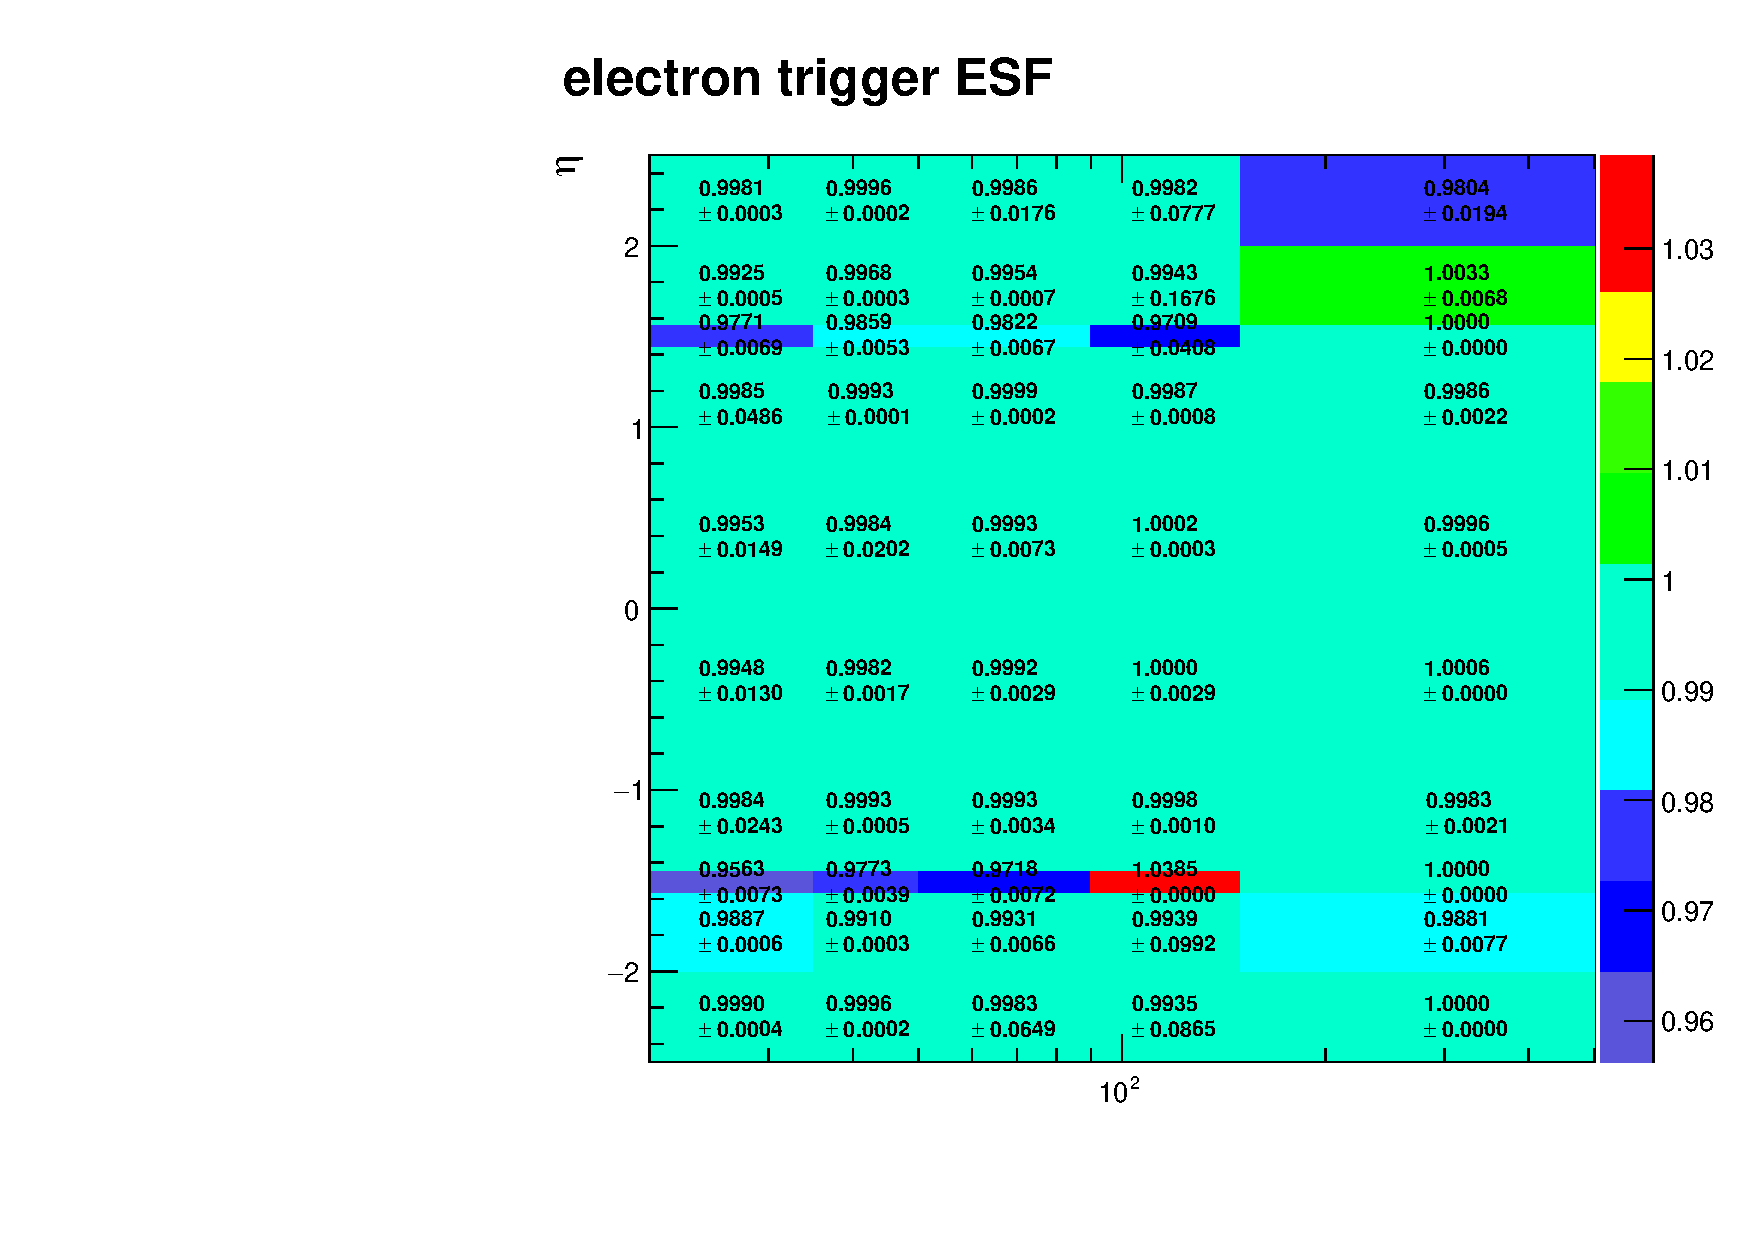
\includegraphics[width=0.49\textwidth]{Figures/egTrigger_TrailingESF.pdf}
 \caption{Trigger efficiency scale factors for the photon (left) and electron (right). }
  \label{fig:egtriggerESF}
\end{figure}


\subsection{$\mu\gamma$ Trigger Performance}

The HLT used in $\mu\gamma$ channel is a combination of two muon-photon cross triggers.
The main HLT is HLT\_Mu17\_Photon30\_CaloIdL\_L1Iso, which is based on L1\_Mu5\_IsoEG20/L1\_Mu5\_IsoEG18 L1 seeds. 
Because of the presence of isolation requirements on L1 EG object, the L1 efficiency has a slower turn-on curve than non-isolated EG triggers.
Thus a second trigger, HLT\_Mu38NoFilterNoVtx\_Photon38\_CaloIdL which has no L1 isolation requirements, is used in logic OR to improve the efficiency.

The $\mu\gamma$ channel trigger efficiency is measured using $Z\rightarrow\mu\mu\gamma$ events selected from SingleMuon dataset. 
HLT\_MuIso24 and HLT\_MuTrkIso24 are used in a logic OR to select events. 
Again, a tag-and-probe method is applied to get pure muon and photon objects. 
The tag is defined as a medium working-point muon which fires one or both of the single muon triggers.
 A second muon and a photon are selected as probes. 
 The probe muon and photon must pass the corresponding offline selections and the $\mu\mu\gamma$ three-body mass must be between 60 GeV and 120 GeV. 
 To ensure that the photon comes from FSR, the muon pair invariant mass is required to be less than 80 GeV. 
 Out of the muon-photon probe pairs, those ones that have both objects matching the trigger objects are selected as the numerator. 
 Figure \ref{fig:mgtriggereff} shows the muon-photon trigger efficiency as a function of photon $p_{T}$ and muon $p_{T}$. 

\begin{figure}[tb]
 \centering
 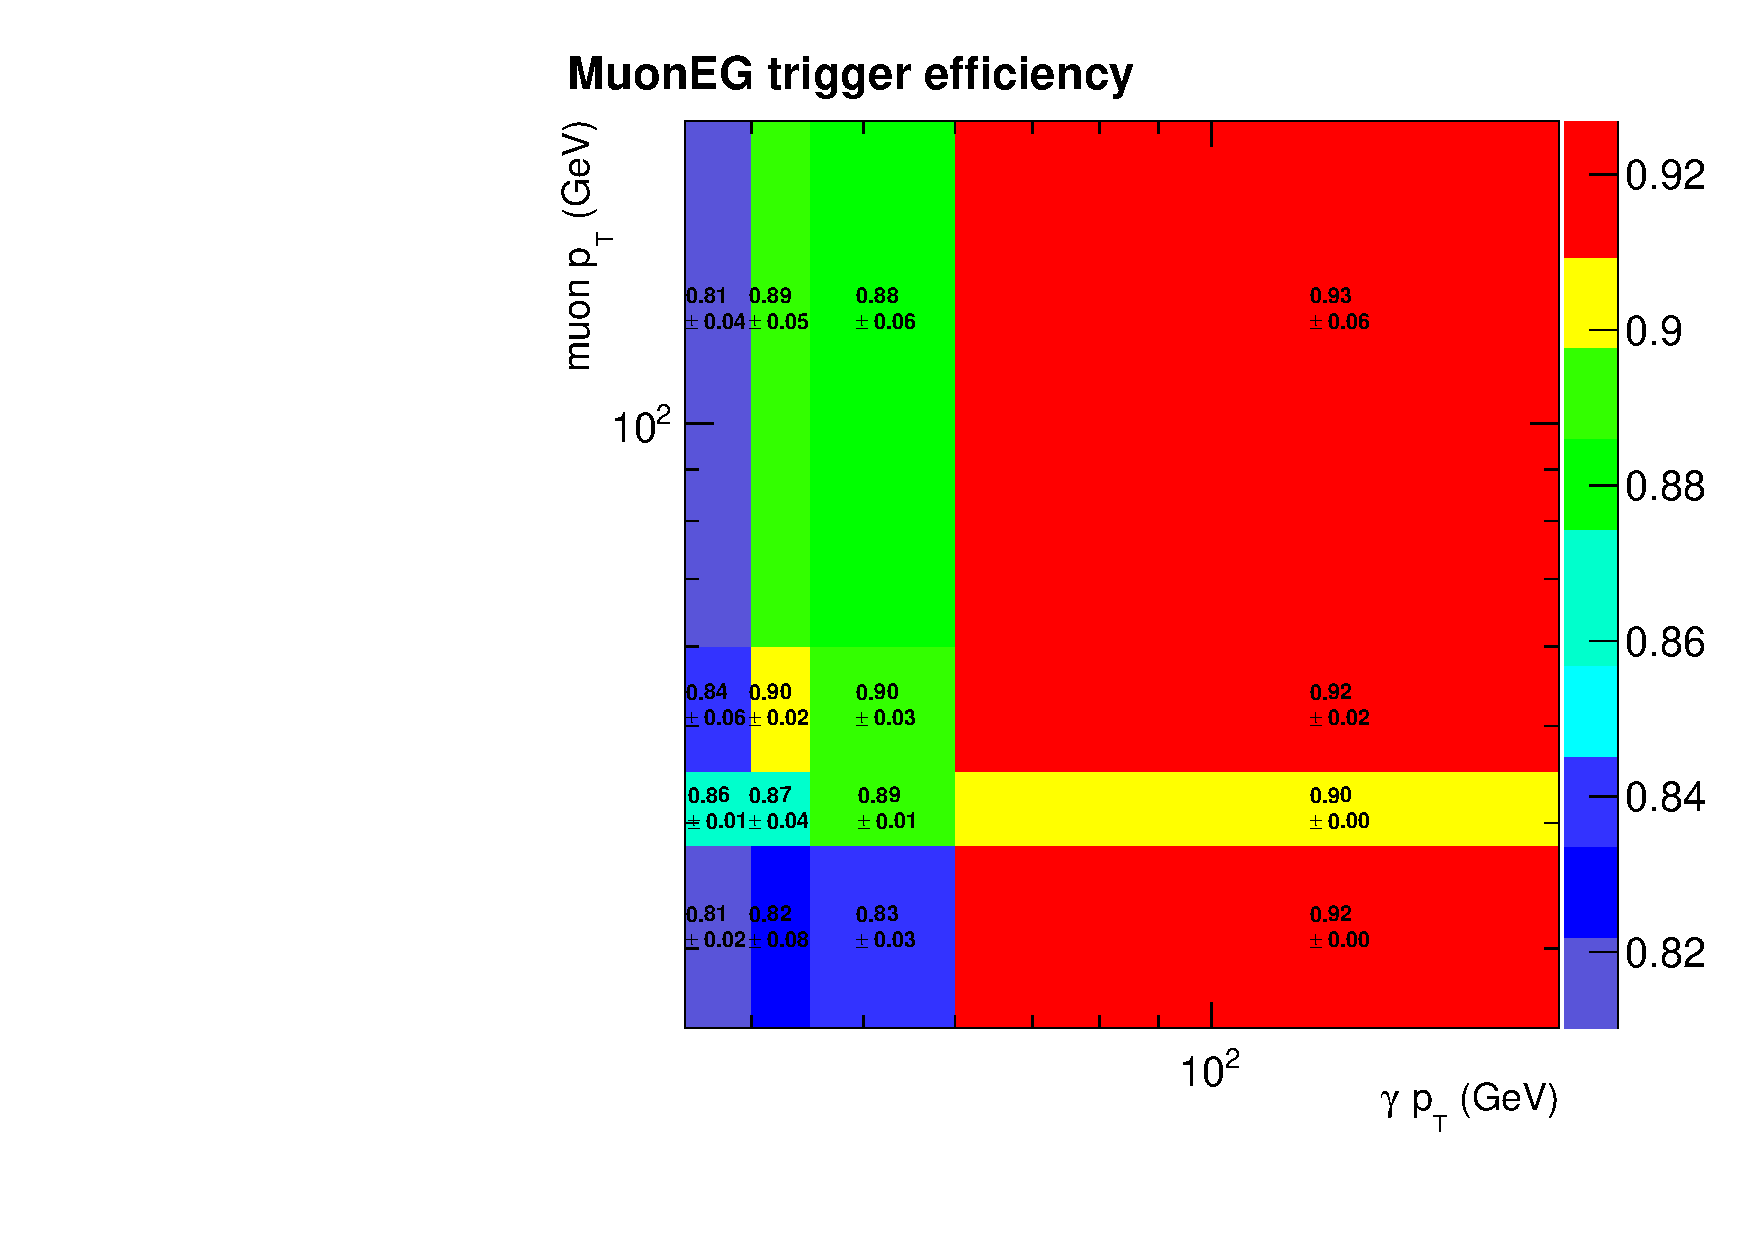
\includegraphics[width=0.8\textwidth]{Figures/mgTrigger_efficiency.pdf}
  \caption{$\mu\gamma$ trigger efficiency as a function of photon and muon $p_{T}$ }
  \label{fig:mgtriggereff}
\end{figure}

The efficiency measurements based on FSR events suffer from low statistics at high $p_{T}$. To cross check the results obtained from $Z\rightarrow\mu\mu\gamma$, we separately measure the muon and photon trigger efficiencies in SinglePhoton and SingleMuon dataset. The discrepancies between these two methods are used as the systematic uncertainties of the $\mu\gamma$ trigger ESF. Figure \ref{fig:mgtriggerESF} shows the muon-photon ESF, along with the uncertainties. 


\begin{figure}[tb]
 \centering
 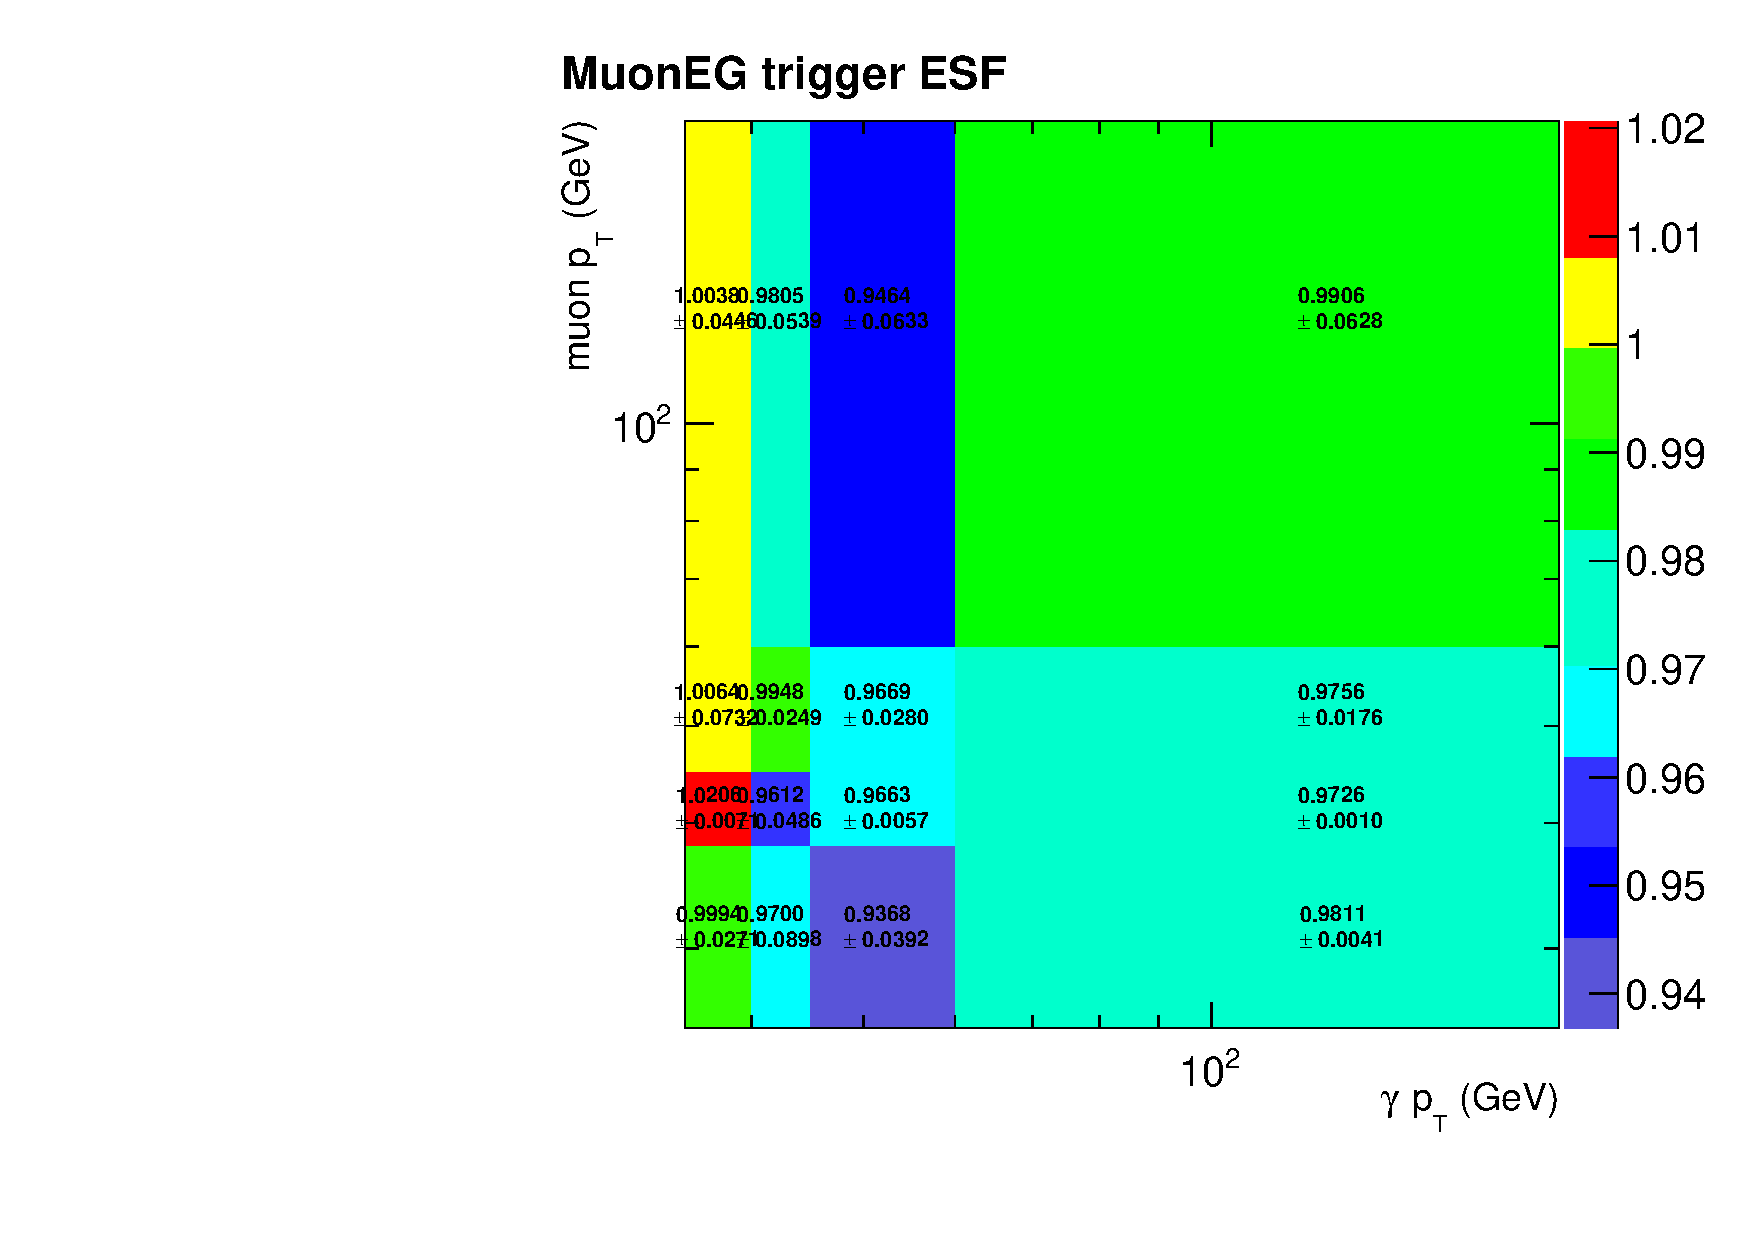
\includegraphics[width=0.8\textwidth]{Figures/mgTrigger_ESF.pdf}
  \caption{$\mu\gamma$ simulation-to-data trigger efficiency scale factor as a function of photon and muon $p_{T}$ }
  \label{fig:mgtriggerESF}
\end{figure}

\end{document}
